%version history since 20221129
%empty page before ad after colofon
%todo inserted pages are not emptu, sometimes numbered
%header footer bars of L/R pages are different
\usepackage{ifthen}%dec2019 macrodefinitions
\usepackage{subfiles}
\newcommand{\onlyinsubfile}[1]{#1}
\newcommand{\notinsubfile}[1]{}
\usepackage[%
    skip=.5\baselineskip plus 2pt,
    %skip=0pt,  %feb 2021
    indent=0pt,
    parfill]{parskip}%dec 2019 n skip=.5\baselineskip plus 2pt
\usepackage[table]{xcolor} %xcolor voor tikz, tbv webgeneratted tables
\usepackage{geometry}%paper size, orientation, margins
%\usepackage{pdflscape}%20080812 oscilloscope
%\usepackage{rotating}%20080812 oscilloscope werkt beter, niet gebruikt
\usepackage{wrapfig}
\usepackage{fancyhdr}%we do have a fancy header
\usepackage{datetime2}%timestamp in the footer
%\usepackage{floatrow}%jun2020 bronvermelding figuren
\usepackage{lastpage}%page N of M
\usepackage{calc}
\usepackage{tikz}%goede plaats?
%\usetikzlibrary{external}%7 jul2020 geheugentekort met mdframes
\usetikzlibrary{babel}%generally good idea, but req'd for issues with catcodes in Tikz (esp quotes, angles)
\usetikzlibrary{calc}% 11 april 2017
\usetikzlibrary{tikzmark}% 12july 2021
\usetikzlibrary{intersections}% 7 mar 18 supergeleiding
\usetikzlibrary{shapes}% 11 april 2017
\usetikzlibrary{arrows,shapes.gates.logic.US,shapes.gates.logic.IEC,calc}%22 juni2020 logic gates
\usetikzlibrary{quotes,angles}%arrow angle alpha in base transform H2

\usepackage{tikzpagenodes}
\usepackage[europeanresistors, RPvoltages]{circuitikz}%15 mar 18 supergeleiding%jun20 update miktech
\usepackage{tikzscale}%15 mar 18 abs scale tikxpicture to marginpar
\usetikzlibrary{decorations.markings}%18 july2018 centered arrowheads qcsuperposition 
\usetikzlibrary{matrix}%25dec2019matrix met pijlen
%\usetikzlibrary{datavisualization.formats.functions}%17-mar-18 pv
\usepackage{pgf-spectra} % 11 april 2017 requires file spectra.data.tex This file is installed in the wrong location.
%should be in:  C:\Program Files\MiKTeX 2.9\tex\latex\pgf-spectra %note: miktex file name database database must be rebuild
\usepackage{pgfplots}
\pgfplotsset{compat=1.13}
\usepackage{marginnote}
\usepackage[framemethod=tikz]{mdframed}
%\usepackage{graphicx} %loaded by tikz
%\usepackage[dvipsnames]{xcolor}   %ook al geladen??
%\usepackage{transparent} %transparent pictures save ink
%\usepackage{layout}%command \layout draws tthe layout of the document
%\usepackage{showframe}                     %show the margins
%use for defining an boxed text experiment
\usepackage{soul}   %highlight text
\sethlcolor{yellow}
\usepackage{lmodern}          %better font rendering
\usepackage[T1]{fontenc}     %8bit
\usepackage[utf8]{inputenc}   %tbv \degree in SIunitx uncommented 26 june 2020
\usepackage[dutch]{babel}%spellchecker
\usepackage{csquotes}%with babel, international quotes, one warning less
\usepackage{verbatim}
\usepackage{amsmath}
\usepackage{amsfonts}
\usepackage{amssymb}
%\usepackage{microtype}% march 2021 
\widowpenalty10000
\clubpenalty10000
%\usepackage{fdsymbol}%dec2019 piste symbols
%\usepackage{marvosym}% \Mobilefone bb84
\usepackage{bbding}%\Phone
\usepackage[gen]{eurosym}%march2020 euro symbol in all typefaces
\usepackage{enumitem}
\setlist{noitemsep}
\setlist[enumerate]{label=\textbf{\alph*}.}
%\usepackage{version}%conditional text (answers)
%\includeversion{solution}
\usepackage{tagging}
\droptag{teach}%!!!!!!!!!!!!!!!!!!!!!!!!!!!!!!!!!!!!
%\usetag{teach}%callouts in environment antwoord
\droptag{eruit}%!!!!!!!!!!!!!!!!!!!!!!!!!!!!!!!!!
%\usetag{eruit}%
\usepackage{qrcode}%jun2020 QRcodes in de marge voor augmented learning
\usepackage[braket,qm]{qcircuit}%24 juni 2018 quantumcomputing conflict with datatool
\usepackage{physics}% 24 juni 2018 quantumcomputing
\usepackage[wby]{callouts}%10 aug 2018 scope image annotation
%\renewcommand{\itemsep}{-1ex}%{4.5pt plus 2.0pt minus 1.0pt}%=default
\usepackage{datatool}%voor printen van certificaten

%\usepackage[font={footnotesize}, labelsep=colon,
%   format=plain]{caption}
%\usepackage{subcaption}
%\renewcommand{\captionlabelfont}{\normal}
\usepackage[margin=10pt,font=small,labelfont=bf,
labelsep=colon]{caption}
%\usepackage{subcaption} %dec2019 figuren naast elkaar
%\captionsetup{
%  figurename={Fig.},
%  justification=raggedright,
%  labelfont={bf},
%  font=small}
\usepackage[binary-units]{siunitx}%getallen blijven bij de eenheid, komma punt probleem en meer
\sisetup{
  list-final-separator={ en },
  list-pair-separator={ en },
  list-separator= {, },
  range-phrase={ tot },
  output-decimal-marker = {,}
  }
\usepackage{blindtext}
%\usepackage{ifoddpage}
%\usepackage[strict]{changepage}%check even odd pg  \whereami adjustwidth jan 2021

%\usepackage{movie15}

%\usepackage{draftwatermark}
%\SetWatermarkText{draft}
%\SetWatermarkScale{1}
%\SetWatermarkColor{red!10}

%-----------------------------------------------
%----25 juni 2020 biblatex erbij
%om referentielijst op te nemen de compilatieinstellingen geupdate
%allereerst miktex packages geupdate (25 jun 2020)
%uitebreide handleiding
%http://ftp.snt.utwente.nl/pub/software/tex/macros/latex/exptl/biblatex/doc/biblatex.pdf
%
%in In texmaker Options>Configure Texmaker
%>Commands: blib(la)tex: biber %
%>quickbuild tweede optie selecteren (was eerste)
%
\usepackage[
    backend=biber,
    style=numeric,%authoryear-icomp,
%    sortlocale=de_DE,
    natbib=true,
%    url=false, 
    doi=true,
%    eprint=false
]{biblatex}
\providecommand{\main}{.}%provide means: define only if not yet defined, so no effect if defined earlier
\addbibresource{\main/bib/nltqc.bib}%ref from subfiles

\usepackage{environ}%solution for unbalanced braces in environments zoals opgave \BODY
%\usepackage[draft]{showkeys}%laat labels zien
\usepackage[final]{showkeys}%laat labels zien!!!!!!!!!!!!!!!!!!!
\renewcommand{\showkeyslabelformat}[1]{%
\fbox{\normalfont\tiny\ttfamily#1}}
\usepackage[strict]{changepage}%check for even odd page command \whereami jan 2021
\usepackage{hyperref}%hyperref moet als laatste package geladen worden
\hypersetup{
    colorlinks=true,
    linkcolor= blue,
    citecolor= blue,
    filecolor= red,
    urlcolor= magenta,
}

%=============no package loads after this line================================

%-----macro definitions--------------------
\newcommand\nogdoen[1]{\textcolor{red}{#1}}
\newcommand\whereami{\checkoddpage\ifoddpage odd\else even\fi}%debug command
%----------------------------------------------------------------------
\renewcommand{\familydefault}{\sfdefault}    %standaardfont
\renewcommand\theContinuedFloat{\alph{ContinuedFloat}}%caption subfigure numbering
\newcommand{\vinger}{\raisebox{-1ex}{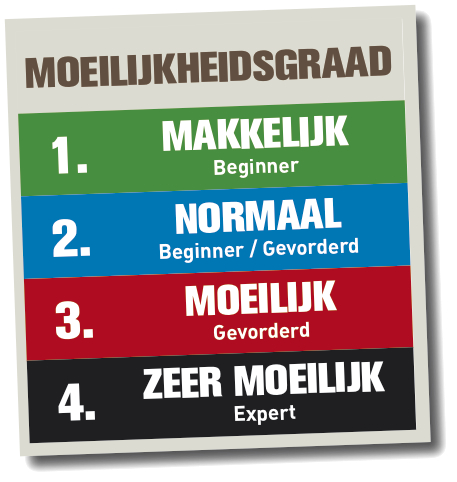
\includegraphics[height=3ex]{../img/pistes.jpg}}\quad}%
%--------------------------------------------
\newcommand*{\lvleasy}{$\textcolor{green}{\text{\LARGE\ensuremath \bullet}}$}
\newcommand*{\lvlnormal}{$\textcolor{blue}{\blacksquare}$}
\newcommand*{\lvldiff}{$\textcolor{black}{\blacklozenge}$}
\newcommand*{\lvlfun}{$\textcolor{red}{\bigstar}$}
\newcommand{\negpar}[1][-1em]{%
  \ifvmode\else\par\fi
  {\parindent=#1\leavevmode}\ignorespaces}
\newcommand*{\easy}{\negpar[-2em] \lvleasy  \hspace*{.5em}}
\newcommand*{\normal}{\negpar[-2em] \lvlnormal \hspace*{.5em}}
\newcommand*{\diff}{\negpar[-2.1em] \lvldiff \hspace*{.4em}}
\newcommand*{\fun}{\negpar[-2.2em] \lvlfun \hspace*{.4em}}

\newcommand*{\vect}[1]{\ensuremath{\vec{#1}}}
\newcommand*{\matr}[1]{\ensuremath{#1}}
%\newcommand*{\port}[1]{\textbf {#1}}
\newcommand*{\port}[1]{\mathversion{bold}\textbf{#1}\mathversion{normal}}

\newcommand*\rot[2]{\rotatebox[origin=c]{#1}{#2} }%filter bB84
%------------------------
%------------define header/footers----------------
\pagestyle{fancy}
%\renewcommand{\chaptermark}[1]{\leftmark{\thechapter.\ #1}}
\renewcommand{\chaptermark}[1]{\markboth{\thechapter.\ #1}{}}
\fancypagestyle{mypage}{%--------definition mypage
\fancyhf{}%clear header and footer
\headheight = 15pt  %minimum=15pt adjust with size of logo (70pt
%\thechapter is nu alleen het nummer
\fancyhead[LO]{Kansen met Quantum}%\rightmark%
\fancyhead[RO]{\leftmark}
\fancyhead[CO]{}%\thechapter
\fancyhead[LE]{\leftmark}%
\fancyhead[RE]{Kansen met Quantum}%\rightmark%
\fancyhead[CE]{}%\thechapter

\fancyfoot[LO, RE]{versie \DTMtoday}
\fancyfoot[C]{\thepage\ of \pageref{LastPage}}
%\fancyfoot[RE,LO]{\whereami}%debug
\textwidth=325pt  %=4.5''
\marginparwidth = 108pt   %108pt=1.5in
\setlength{\evensidemargin}{\marginparwidth + \marginparsep}
\addtolength\headwidth{\marginparwidth + \marginparsep}

\newlength{\fullwidth}
\setlength{\fullwidth}{\marginparwidth + \marginparsep+\textwidth}
\newlength{\fullmargin}
\setlength{\fullmargin}{\marginparwidth + \marginparsep}

\renewcommand{\headrulewidth}{5pt}
\renewcommand{\footrulewidth}{2pt}
\fancyheadoffset[LE,RO]{\marginparwidth + \marginparsep}
\fancyfootoffset[LE,RO]{\marginparwidth + \marginparsep}

}%--------end definition mypage
\pagestyle{mypage}
%----------

%\title{Kansen met Quantum}%hoort bij maketitle
%starred version cannot contain parbreaks
\newcommand*{\hrefnote}[2]{%href in de text, automatisch voetnoot 
\href{#1}{#2}\footnote{\url{#1}}}

\newcommand*{\hrefqr}[3][0cm]{%href in de text, QR code in de marge
\href{#2}{#3}\marginnote{\vskip #1%changed marginpar to marginnote (no floats)
\qrcode[height=.5\marginparwidth]{#2}\\ {\scriptsize #3}}}

\tikzstyle{extra} = [draw=black, 
  very thick,
  rectangle,
  rounded corners,
  inner xsep=3pt, inner ysep=10pt]
\tikzstyle{extratitle} = [fill=red!10, text=black, right=10pt]

%minipage en tikz misschien niet de beste oplossing
%zie https://hbfs.wordpress.com/2015/03/17/a-simple-latex-example-environment/
%-gaat over pagine einde
%
%enorm groot kader vraagt extra geheugen 
%voeg toe in pdflatex compile opdracht:  --extra-mem-bot=10000000

\global\mdfdefinestyle{wiskader}{%
linecolor=blue!80,
linewidth=2pt,
%backgroundcolor=blue!8,
rightline=false,
topline=false,
bottomline=false,
innerleftmargin=5,
innerrightmargin=5,
frametitlerule=false,
%frametitlerulecolor=green,
frametitlebackgroundcolor=blue!20,
frametitlerulewidth=2pt
}

\newcounter{expetel}[chapter]\setcounter{expetel}{0}
\renewcommand{\theexpetel}{\thechapter.\arabic{expetel}}
\NewEnviron{experiment}[2][green]{%
%\refstepcounter{expetel}%220114 geen nummering
\ifstrempty{#2}%
  {
  \mdfsetup{%
    frametitle={%
    \tikz[baseline=(current bounding box.east),outer sep=0pt]
    \node[anchor=east,rectangle,fill=#1!40]
%    {\strut Experiment~\theexpetel~#2};},
    {\strut #2};},%220114 geen nummering geen experiment
    innertopmargin=10pt,linecolor=#1!40,%
    backgroundcolor=#1!10,
    linewidth=2pt,topline=true,%
    frametitlebackgroundcolor=#1!10,
    frametitleaboveskip=-5pt,%\dimexpr-\ht\strutbox\relax%oorzaak foute breaks
    nobreak=true
    }
    }% ifempty
  {\mdfsetup{%
    frametitle={%
    \tikz[baseline=(current bounding box.east),outer sep=0pt]
    \node[anchor=east,rectangle,fill=#1!40]
%    {\strut Experiment~\theexpetel~#2};},
    {\strut #2};},%220114 geen nummering geen experiment
    innertopmargin=10pt,linecolor=#1!40,%
    backgroundcolor=#1!10,
    linewidth=2pt,topline=true,%
    frametitlebackgroundcolor=#1!10,
    frametitleaboveskip=-5pt,%\dimexpr-\ht\strutbox\relax%oorzaak foute breaks
    nobreak=true
    }}%if not empty
\begin{mdframed}[]\relax%
\BODY
\end{mdframed}}

\NewEnviron{opdracht}[1][green]{%
\refstepcounter{expetel}%
\mdfsetup{%
  frametitle={%
  \tikz[baseline=(current bounding box.east),outer sep=0pt]
  \node[anchor=east,rectangle,fill=#1!40]
  {\strut Opdracht~\theexpetel};},
  innertopmargin=10pt,linecolor=#1!40,%
  backgroundcolor=#1!10,
  linewidth=2pt,topline=true,%
  frametitlebackgroundcolor=#1!10,
  frametitleaboveskip=-5pt,%\dimexpr-\ht\strutbox\relax%oorzaak foute breaks
  nobreak=true
  }
\begin{mdframed}[]\relax%
\BODY
\end{mdframed}}

\NewEnviron{opdrachtlang}[1][green]{%
\refstepcounter{expetel}%
\mdfsetup{%
  frametitle={%
  \tikz[baseline=(current bounding box.east),outer sep=0pt]
  \node[anchor=east,rectangle,fill=#1!40]
  {\strut Opdracht~\theexpetel};},
  innertopmargin=10pt,linecolor=#1!40,%
  backgroundcolor=#1!10,
  linewidth=2pt,topline=true,%
  frametitlebackgroundcolor=#1!10,
  frametitleaboveskip=-5pt,%\dimexpr-\ht\strutbox\relax%oorzaak foute breaks
  skipabove={1.2\baselineskip},% toegevoegd vanwege vreemde pagebreaks
  innertopmargin={1.2\baselineskip},%  toegevoegd vanwege vreemde pagebreaks
  nobreak=false
  }
\begin{mdframed}[]\relax%
\BODY
\end{mdframed}}

\iffalse%========oud===========
\NewEnviron{experiment}[1][green]{\refstepcounter{expetel}%
\vspace{1em plus 1em}%
\begin{tikzpicture}
\node [extra, fill=#1!10] (box){%
\begin{minipage}{\dimexpr\linewidth-2\fboxrule-2\fboxsep\relax}
noindent\textbf{Problem~\theHexpetel}
\BODY
\end{minipage}};%end node
\node [extratitle] at (box.north west) {\textbf{Experiment~\theexpetel}};
\end{tikzpicture}
\vspace{1em plus 1em}%
}%---

\NewEnviron{opdracht}[1][green]{\refstepcounter{expetel}%
\vspace{1em plus 1em}%
\begin{tikzpicture}
\node [extra, fill=#1!10] (box){%
\fcolorbox{#1!10}{#1!10}{%
\parbox{.95\textwidth}{%
{\BODY}
}}
};%node
\node [extratitle] at (box.north west) {\textbf{Opdracht~\theexpetel}};
\end{tikzpicture}%
\vspace{1em plus 1em}%
}
\fi%================oud=====================

\NewEnviron{antwoord}[1][0cm]{\tagged{teach}{%
\marginnote{\vskip #1%
\fcolorbox{red}{yellow}{%
\parbox{0.9\marginparwidth}{%
{\raggedright
\footnotesize{%
{\BODY}
}}}}}}}


\newcommand\notepadlines[1][5]{
\checkoddpage\ifoddpage 
    \def\xoff{0pt}
  \else 
    \def\xoff{-\marginparsep-\marginparwidth}
  \fi
\def\lines{#1}
\begin{adjustwidth}{\xoff}{0pt}
\noindent\begin{tikzpicture}[remember picture]%
%\begin{scope}
%   \node[draw] at (0, 0)   (a) {};
   \node (0,0){\mbox{\parbox[b][0.71cm*\lines][b]{15mm}{%
    \begin{tikzpicture}[remember picture,overlay]%, xshift=\xoff,yshift=0cm]
        \definecolor{notepadrule}{RGB}{168,230,230}
        \definecolor{leftdivider}{RGB}{255,122,122}
        \tikzset{normal lines/.style={notepadrule, thin}} 
        \tikzset{margin lines/.style={leftdivider, thick}} 
        \foreach \y in {0,1, ..., \lines}
            \draw[style=normal lines](0, 0.71*\y) -- (\fullwidth, 0.71*\y);
        \draw[style=margin lines] (2cm,0)--(2cm, \lines*.71);
    \end{tikzpicture}
  }}};
%\end{scope}
\end{tikzpicture}
\end{adjustwidth}
}
%tbv strikethrough math (termen wegstrepen) met een label
\tikzset{
main node/.style={inner sep=0,outer sep=0},
strike out/.style={shorten <=-.2em,shorten >=-.2em,overlay, red, thick}
}
\newcommand{\xcancelto}[1]{\tikz[baseline=(N.base)]{
  \node[main node](N){$\mathrm{#1}$};
  \draw[strike out,-]  (N.south east) -- (N.north west);
  \draw[strike out,-]  (N.south west) -- (N.north east);
}}


%space squeezing:
%https://robjhyndman.com/hyndsight/squeezing-space-with-latex/
%--------------------------
\makeatletter%get rid of text chapter
\def\@makechapterhead#1{%
  \vspace*{20\p@}%was50, beetje hoger op de pagina
  {\parindent \z@ \raggedright \normalfont
    \ifnum \c@secnumdepth >\m@ne
      \if@mainmatter
        %\huge\bfseries \@chapapp\space \thechapter
        \Huge\bfseries \thechapter.\space%
        %\par\nobreak
        %\vskip 20\p@
      \fi
    \fi
    \interlinepenalty\@M
    \Huge \bfseries #1\par\nobreak
    \vskip 30\p@%was40
  }}
\makeatother
%--------------------------
